\documentclass[11pt]{article}
\usepackage[T1]{fontenc}
\usepackage[utf8]{inputenc}
\usepackage{lmodern,amsmath,amssymb,amsthm,booktabs,array}
\usepackage[margin=27mm]{geometry}
\usepackage{tikz}
\usepackage{needspace}
\usetikzlibrary{arrows.meta}
\usepackage[colorlinks=true,allcolors=blue]{hyperref}
\hypersetup{pdftitle={An exact specified-state collision threshold in a binary automaton family},pdfauthor={Qichao Wang},pdfsubject={Exact pair distances in synchronizing automata},pdfkeywords={synchronizing automata, compress-with-another threshold, pair automaton}}
\newtheorem{theorem}{Theorem}
\newtheorem{lemma}[theorem]{Lemma}
\newtheorem{proposition}[theorem]{Proposition}
\newtheorem{corollary}[theorem]{Corollary}
\newcommand{\dist}{\operatorname{dist}}
\newcommand{\M}[1]{M_{#1}}
\newcommand{\Ost}[1]{O_{#1}}
\newcommand{\pair}[2]{\{#1,#2\}}
\title{An exact specified-state collision threshold\\ in a binary automaton family}
\author{Qichao Wang\\Hebei University of Technology}
\date{3 October 2026}
\begin{document}
\maketitle
\begin{abstract}
For a specified state of a synchronizing automaton, the compress-with-another threshold is the shortest length of a word that merges it with any other state. We determine this threshold for the corrected binary family in Figure~3 of Szyku\l a's survey of open problems. For every $p\geq3$, the family has $n=3p$ states and the distinguished state satisfies $\mu(q_0)=4p=4n/3$, attained by $(ba)^p(ab)^p$. A self-contained pair-automaton proof establishes the lower bound using two entrance potentials and an excluded region, including the endpoint case $p=3$. An explicit reset word of length $3p^2+4p-1$ proves synchronization for every parameter. The family therefore realizes the proposed $4n/3$ specified-state threshold and requires a leading constant of at least $4/3$ in any uniform linear bound, even for binary strongly connected automata whose letters have corank one.
\end{abstract}

\section{Introduction}
A complete deterministic semiautomaton $(Q,\Sigma,\delta)$ is synchronizing if some word maps $Q$ to a singleton. Such a word is a reset word, and the reset threshold $\operatorname{rt}(\mathcal A)$ is its minimum length. We use right actions, writing $qw=\delta(q,w)$, and count word length in original letters. For a state $q$, put
\[
 \mu(q)=\min\{|w|:qw=rw\text{ for some }r\in Q\setminus\{q\}\}.
\]
The minimum is finite in a synchronizing automaton. It concerns one collision involving a specified initial state, whereas a reset word must merge all initial states.

Szyku\l a~\cite{szykula} asks whether $\mu(q)=O(n)$ in every strongly connected synchronizing $n$-state automaton. His Figure~3, attributed there to D\.{z}yga's 2018 master's thesis~\cite{dzyga}, gives a binary family on $3k+6$ states proposed to attain $4n/3$. Conjecture~8 asserts synchronization of the family and this specified-state threshold. For general background we refer to Volkov~\cite{volkov}; the \v Cern\'y conjecture~\cite{cerny}, asking for reset words of length at most $(n-1)^2$, remains open. We prove the proposed threshold and synchronization for the completed transition definition below.

We use $p=k+2\geq3$ and state the corrected transitions in full. The initial $b$-edge and the terminal matching edges complete the published description. The word printed in Conjecture~8 of the published version, $(ab)^p a(ab)^p$, has $4p+1$ letters; the corrected witness $(ba)^p(ab)^p$ has $4p$ letters and merges $q_0$ with $q_2$. We use the EPTCS publication and public arXiv v1 of~\cite{szykula} as the source of the original figure and conjecture.

We track a pair of distinct states until its first collision. Each letter merges only one pair, so the threshold reduces to the distance from an initial pair containing $q_0$ to one of these two kernel pairs. Two time lower bounds, propagated across complete lists of incoming transitions, show that neither kernel pair can be reached earlier than claimed. An invariant excludes otherwise possible shortcuts. The argument applies to arbitrary words and initial partners; a separate image-shrinking construction proves synchronization.

An earlier release by Korea Superintelligence Labs, generated by Machina Mathematica~\cite{machina}, established the all-parameter upper witness and reported exact finite computations. Lawson subsequently announced and published a candidate all-parameter proof, including a pair-space certificate and a separate synchronization construction~\cite{modal12,modal30}. His displayed reset word has length $4p^2+6p$; the construction here gives the smaller bound $3p^2+4p-1$. Szyku\l a has also informed the author of other independently communicated proofs. We make no priority claim. Our contribution is the self-contained entrance-potential proof and explicit reset construction presented below.

\section{The corrected Figure~3 family}
Let $\mathcal A_p$ have $Q=\{q_0,\ldots,q_{3p-1}\}$ and alphabet $\{a,b\}$. The complete definition is conveniently given by matchings and three exceptional edges. Letter $a$ fixes $q_0$, swaps $q_{2j-1}$ and $q_{2j}$ for $1\leq j\leq p-1$, and has
\[
 q_{2p-1}a=q_{2p},\qquad q_{2p}a=q_{2p+1},\qquad q_{2p+1}a=q_3.
\]
On $q_{2p+2},\ldots,q_{3p-1}$ it swaps successive pairs starting at the even index $2p+2$; an unmatched last state is fixed. Letter $b$ swaps $q_{2j}$ and $q_{2j+1}$ for $0\leq j\leq p-1$, has $q_{2p}b=q_2$, and swaps successive pairs on $q_{2p+1},\ldots,q_{3p-1}$ starting at $2p+1$, again fixing an unmatched last state. These rules also specify $q_0b=q_1$.

For the proof write
\[
 \M i=q_i\ (0\leq i\leq2p),\qquad
 \Ost h=q_{4p-h}\ (p+1\leq h\leq2p-1).
\]
The outer coordinate runs in the reverse direction. Away from the exceptions, on either branch letter $a$ increases an odd coordinate by one and decreases an even coordinate by one; $b$ does the opposite. At the outer bottom $h=p+1$, the decreasing letter fixes the state. It is $a$ when $p+1$ is even and $b$ when $p+1$ is odd. The remaining exceptional rules are
\begin{equation}\label{eq:exceptions}
 \M0a=\M0,\quad \M{2p}a=\Ost{2p-1},\quad
 \M{2p}b=\M2,\quad \Ost{2p-1}a=\M3.
\end{equation}

\begin{figure}[ht]
\centering
% Original schematic, drawn from the completed transition definition.
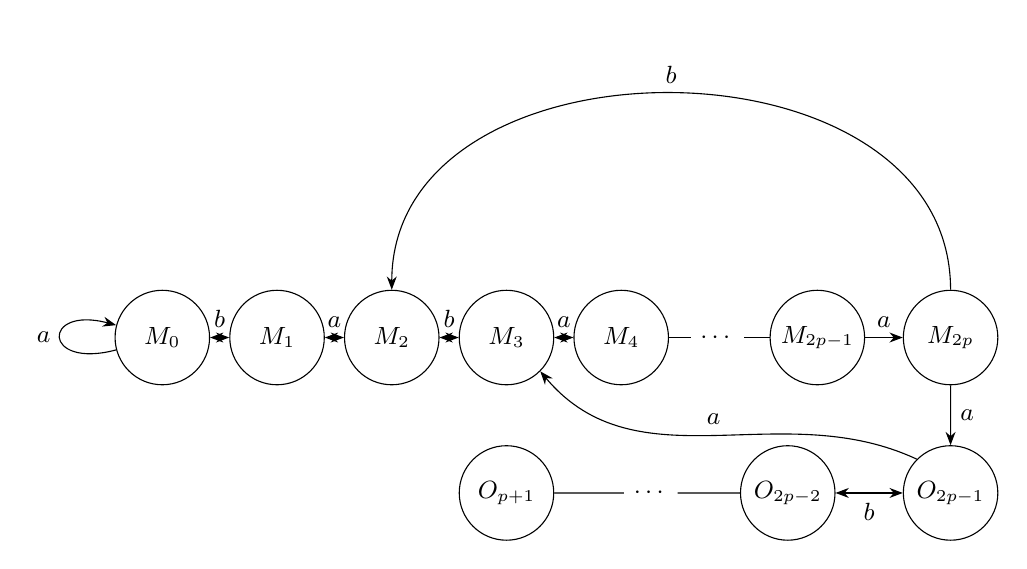
\begin{tikzpicture}[>=Stealth,scale=.94,every node/.style={font=\small},
 state/.style={draw,circle,minimum size=12mm,inner sep=0pt}]
\node[state] (m0) at (0,0) {$M_0$};
\node[state] (m1) at (1.55,0) {$M_1$};
\node[state] (m2) at (3.1,0) {$M_2$};
\node[state] (m3) at (4.65,0) {$M_3$};
\node[state] (m4) at (6.2,0) {$M_4$};
\node (dots) at (7.5,0) {$\cdots$};
\node[state] (mpm) at (8.85,0) {$M_{2p-1}$};
\node[state] (mp) at (10.65,0) {$M_{2p}$};
\draw[<->] (m0)--node[above]{$b$}(m1);
\draw[<->] (m1)--node[above]{$a$}(m2);
\draw[<->] (m2)--node[above]{$b$}(m3);
\draw[<->] (m3)--node[above]{$a$}(m4);
\draw (m4)--(dots);\draw (dots)--(mpm);
\draw[->] (mpm)--node[above]{$a$}(mp);
\node[state] (ot) at (10.65,-2.1) {$O_{2p-1}$};
\node[state] (on) at (8.45,-2.1) {$O_{2p-2}$};
\node (od) at (6.6,-2.1) {$\cdots$};
\node[state] (ob) at (4.65,-2.1) {$O_{p+1}$};
\draw[->] (mp)--node[right]{$a$}(ot);
\draw[<->] (ot)--node[below]{$b$}(on);
\draw (on)--(od);\draw (od)--(ob);
\draw[->] (ot.north west) to[out=155,in=-50] node[above,sloped]{$a$}(m3.south east);
\draw[->] (mp.north) to[out=90,in=90,looseness=1.2] node[above]{$b$}(m2.north);
\draw[->] (m0) to[loop left] node[left]{$a$}(m0);
\end{tikzpicture}
\caption{The corrected Figure~3 family~\cite{szykula}, shown schematically for $p\geq5$. Unlabelled segments continue the alternating matchings. The outer bottom $O_{p+1}$ is fixed by its decreasing letter. For $p=4$, the outer branch is $O_7,O_6,O_5$ with no intermediate vertex; for $p=3$, it is $O_5,O_4$ and the displayed labels $O_{2p-2}$ and $O_{p+1}$ denote the same vertex. The transition rules in the text apply in every case.}
\end{figure}

Both letters have rank $3p-1$. Indeed, their only double fibers are
\begin{equation}\label{eq:kernels}
 a^{-1}(\M3)=\pair{\M4}{\Ost{2p-1}}=K_a,
 \qquad b^{-1}(\M2)=\pair{\M3}{\M{2p}}=K_b.
\end{equation}
Each letter misses one image state: $a$ misses $\M{2p-1}$ and $b$ misses $\M{2p}$. All other fibers are singletons.
The underlying directed graph is strongly connected. The main matchings connect $\M0,\ldots,\M{2p-1}$ in both directions, the final main $a$-edge reaches $\M{2p}$, and $a$ then enters the outer branch. Its matchings connect every outer state in both directions, and its top returns to $\M3$; $\M{2p}b=\M2$ also returns to the main chain.

\section{Exact pair distances and the threshold}
The unordered pair graph has vertex set $\binom Q2$. It has a directed edge $P\xrightarrow{x}Px$ for $x\in\{a,b\}$ whenever $|Px|=2$; collapsing edges are omitted. Set
\[
 S_p=\{\pair{\M0}{q}:q\in Q\setminus\{\M0\}\}.
\]
Distance from $S_p$ means the minimum over its vertices. A first collision must use a kernel pair, so
\begin{equation}\label{eq:reduction}
 \mu(q_0)=1+\min\{\dist(S_p,K_a),\dist(S_p,K_b)\}.
\end{equation}

\begin{lemma}\label{lem:dist}
For every $p\geq3$,
\[
 \dist(S_p,K_b)=4p-1,\qquad \dist(S_p,K_a)=4p.
\]
\end{lemma}
\begin{proof}
We prove the lower bounds first. Fix an arbitrary path $P_0\xrightarrow{x_1}P_1\xrightarrow{x_2}\cdots\xrightarrow{x_\ell}P_\ell$ in the distinct-pair graph, where $P_0\in S_p$ and $x_t\in\{a,b\}$. All time bounds refer to its vertex $P_t$ after $t$ original letters.

\paragraph{1. The index bound and excluded region.}
Every original state index increases by at most one in one letter. The particle that started at $q_0$ consequently has index at most the elapsed time $t$. For the current pair $P_t$ this gives
\begin{equation}\label{eq:index}
 t\geq\min\{i:q_i\in P_t\}.
\end{equation}
Let $J$ consist of opposite-parity main pairs whose coordinate sum exceeds $2p+1$. The only reachable member of $J$ is $K_b$.
To see this, an ordinary matching step on an opposite-parity pair preserves its sum, and an ordinary step on a same-parity pair preserves that parity type. A pair involving the fixed $\M0$ cannot acquire a sum above $2p+1$. The $b$-jump from $\M{2p}$ lands at $\M2$; its other main image is at most $\M{2p-1}$. Hence the resulting main-pair coordinate sum is at most $2+(2p-1)=2p+1$, so it cannot enter $J$, which requires a strictly larger sum. The $a$-step from $\M{2p}$ leaves the main branch.

The terminal edge $\M{2p-1}a=\M{2p}$ also requires attention. A target in $J$ containing $\M{2p}$ has the form $\pair{\M{2p}}{\M j}$ with odd $j\geq3$. For $5\leq j\leq2p-3$, its only $a$-preimage is $\pair{\M{2p-1}}{\M{j+1}}$, already in $J\setminus\{K_b\}$ since its sum is $2p+j>2p+1$. The remaining odd endpoint $j=2p-1$ has no $a$-preimage. For $j=3$, the preimage using $\M4$ is likewise already in $J\setminus\{K_b\}$, while $\pair{\M{2p-1}}{\Ost{2p-1}}a=K_b$. An outer-to-main step lands at $\M3$, and an opposite-parity sum above $2p+1$ requires its other image to be $\M{2p}$, exactly the case just treated. Two outer states cannot both enter the main branch in one letter. Finally, $K_ba=K_a$, whereas $|K_bb|=1$. No initial pair lies in $J$, and no edge from outside $J\setminus\{K_b\}$ enters that set. This proves the invariant by induction. Call a pair \emph{admissible} if it is outside $J\setminus\{K_b\}$.

\Needspace{8\baselineskip}
\paragraph{2. The first entrance potential.}
Put
\[
 C=\{\pair{\M x}{\M{2p+1-x}}:1\leq x\leq p\},
 \qquad \phi_C(\pair{\M x}{\M{2p+1-x}})=2p-2+|x-3|.
\]
No initial pair lies in $C$. Each internal edge changes the smaller coordinate by at most one, so the potential increases by at most one. The complete list of admissible entrances from outside $C$ is
\begin{center}\small
\begin{tabular}{@{}cllc@{}}\toprule
Letter & Source & Target & Source-time bound\\\midrule
$a$ & $\pair{\M{2p-3}}{\Ost{2p-1}}$ & $\pair{\M3}{\M{2p-2}}$ & $2p-3$\\
$b$ & $\pair{\M{2p-2}}{\M{2p}}$ & $\pair{\M2}{\M{2p-1}}$ & $2p-2$\\\bottomrule
\end{tabular}
\end{center}
Here and below source-time bounds concern arrival before the entering letter. Both follow from~\eqref{eq:index}; after adding one they equal the target potential. For completeness of the list, an ordinary inverse matching preserves the opposite-parity sum, hence gives a source in $C$. The exceptional $a$-fiber at $\M3$ allows the first outer source displayed above. The exceptional $b$-fiber at $\M2$ allows the second source. Targets containing $\M{2p}$ have no $b$-preimage, and those containing $\M{2p-1}$ have no $a$-preimage. The fixed $\M0$ cannot occur in $C$. These exhaust the exceptional inverse fibers. Thus induction on the path, including any exits and reentries, proves
\begin{equation}\label{eq:C}
 P_t\in C\ \Longrightarrow\ t\geq\phi_C(P_t),
 \qquad \dist(S_p,\pair{\M1}{\M{2p}})\geq2p.
\end{equation}

\paragraph{3. The reflected entrance potential.}
Consider the disjoint tracks
\[
 A=\{\pair{\M x}{\Ost{2p+1-x}}:2\leq x\leq p\},\qquad
 E=\{\pair{\M x}{\Ost x}:p+1\leq x\leq2p-1\}.
\]
For $H=A\cup E$ set $\phi_H=2p-1+x$, where $x$ is the main coordinate. No initial pair lies in $H$. Ordinary internal edges change $x$ by one. At the outer bottom, its decreasing letter exchanges $A$ at $x=p$ with $E$ at $x=p+1$; this also changes the potential by one. All admissible entrances from outside $H$ are
\begin{center}\small
\begin{tabular}{@{}ccllc@{}}\toprule
Letter & Parameter & Source & Target & Source-time bound\\\midrule
$a$ & all $p$ & $\pair{\M1}{\M{2p}}$ & $\pair{\M2}{\Ost{2p-1}}$ & $2p$\\
$b$ & all $p$ & $\pair{\M{2p}}{\Ost{2p-2}}$ & $\pair{\M2}{\Ost{2p-1}}$ & $2p$\\
$a$ & $p\geq4$ & $\pair{\Ost{2p-1}}{\Ost{2p-3}}$ & $\pair{\M3}{\Ost{2p-2}}$ & $2p+1$\\
$a$ & $p=3$ & $\pair{\Ost5}{\Ost4}$ & $\pair{\M3}{\Ost4}$ & $7$\\\bottomrule
\end{tabular}
\end{center}
The first bound is~\eqref{eq:C}; the others follow from~\eqref{eq:index}. Adding one gives $\phi_H$ at each target.

We check completeness uniformly. In the interior of $A$, the coordinates have opposite parity, so both forward and inverse matchings preserve their sum. In the interior of $E$, the equal coordinates move together. At the outer bottom the fixed coordinate joins precisely the two tracks just described. At the outer top, $a^{-1}(\Ost{2p-1})=\{\M{2p}\}$: target main coordinate $2$ gives the first entrance, whereas the top target in $E$ has main coordinate $2p-1$ and no $a$-preimage. Under $b$, the double fiber at $\M2$ gives the second entrance; its other source stays in $H$. To enter from two outer states under $a$, the main image must be $\M3$, hence the target is the $x=3$ member of $A$. Its ordinary outer preimage is $\Ost{2p-3}$ for $p\geq4$. For $p=3$, $h=4$ is the bottom and is fixed by $a$, so that preimage is instead $\Ost4$. These are the last two rows. The missing main images and the remaining ordinary inverse matchings give no further entrances. Therefore
\begin{equation}\label{eq:H}
 P_t=\pair{\M x}{\Ost h}\in H\ \Longrightarrow\ t\geq\phi_H(P_t)=2p-1+x,
 \qquad \dist(S_p,\pair{\M{2p-1}}{\Ost{2p-1}})\geq4p-2.
\end{equation}
For $p=3$, the exceptional entrance gives the same target-time bound, $8$; the top of $E$ is reached no earlier than time $10$.

\paragraph{4. Entrance into the kernel regions.}
There is only one admissible incoming edge to $K_b$:
\begin{equation}\label{eq:Kbentry}
 \pair{\M{2p-1}}{\Ost{2p-1}}\xrightarrow{a}K_b.
\end{equation}
Indeed, $b$ misses $\M{2p}$, and the other $a$-preimage is $\pair{\M4}{\M{2p-1}}$, in $J\setminus\{K_b\}$. Equation~\eqref{eq:H} now yields $\dist(S_p,K_b)\geq4p-1$.

To control $K_a$ define
\[
 B=\{\pair{\M x}{\Ost{2p+3-x}}:4\leq x\leq p+2\},\qquad
 F=\{\pair{\M{h+2}}{\Ost h}:p+1\leq h\leq2p-2\}.
\]
These tracks are disjoint. Their union $U$ contains $K_a$ and no initial pair. Its only admissible entrance from outside $U$ is the $a$-transition from $K_b$ to $K_a$. In fact, ordinary inverse matchings preserve the sum $2p+3$ in $B$, or the difference $2$ in $F$. At the outer bottom the decreasing letter joins $B$ at main coordinate $p+2$ to $F$ at main coordinate $p+3$. The only $U$-target containing the outer top is the $x=4$ member of $B$, namely $K_a$, whose $a$-preimage is $K_b$. A $b$-jump lands at $\M2$, and an outer-to-main $a$-jump at $\M3$, whereas every main coordinate in $U$ is at least $4$. Targets with main coordinate $2p$ have no $b$-preimage; those with main coordinate $2p-1$ have no $a$-preimage. The other top endpoint of $F$, with coordinates $(2p,2p-2)$, has its ordinary $a$-preimage in $F$ for $p\geq4$, and in $B$ for $p=3$. Thus the list exhausts both endpoints and all exceptional fibers, also when $p=3$ and $F$ has only one member.

Every path reaching $U$ has a first entrance immediately preceded by a visit to $K_b$. Hence its first entrance has length at least $4p$, and later visits cannot occur earlier. This proves $\dist(S_p,K_a)\geq4p$. A final $b$-collapse costs at least $4p$, and a final $a$-collapse at least $4p+1$.

\paragraph{5. Matching paths and the upper word.}
Put $c=ba$ and $u=ab$. Direct substitution in the transition rules gives cycles, in the displayed order,
\begin{equation}\label{eq:cycles}
 \begin{aligned}
 R&=(\M0,\M2,\M4,\ldots,\M{2p},\M1) &&\text{under }c,\\
 T&=(\M0,\M1,\M3,\ldots,\M{2p-1},\M2) &&\text{under }u.
 \end{aligned}
\end{equation}
Both have length $p+2$. In particular $\pair{\M0}{\M2}c^p=\pair{\M{2p}}{\M1}$ and $\M1u^p=\M2$. The $u$-chain starting at $\M{2p}$ visits the even-indexed outer states upwards, reflects at the last original state, visits the odd-indexed outer states downwards, and then reaches $\M2$. It consists of $\M{2p}$ and all $p-1$ outer states, so its entrance length is $p$. Consequently
\begin{equation}\label{eq:upper}
 \pair{q_0}{q_2}(ba)^p(ab)^p=\{q_2\}.
\end{equation}
Immediately before the last $a$ in this word, the pair is $\pair{\M{2p-1}}{\Ost{2p-1}}$. After that $a$ it is $K_b$, and the final $b$ collapses it. These pairs are distinct until the last letter: an earlier collision would persist and contradict the distinct penultimate pair. Thus the prefix of length $4p-1$ reaches $K_b$ in the pair graph. Appending $a$, instead of the collapsing $b$, reaches $K_a$ at length $4p$. This proves both upper distance bounds.
\end{proof}

\begin{theorem}\label{thm:main}
For every $p\geq3$, the corrected Figure~3 automaton $\mathcal A_p$ on $n=3p$ states satisfies
\[
 \mu(q_0)=4p=\frac{4n}{3}.
\]
The word $(ba)^p(ab)^p$ is a shortest word compressing $q_0$ with another state; it merges $q_0$ and $q_2$ at $q_2$.
\end{theorem}
\begin{proof}
Combine Lemma~\ref{lem:dist} with~\eqref{eq:reduction} and~\eqref{eq:upper}.
\end{proof}
This proves the specified-state threshold assertion of Conjecture~8 for the corrected family.

\section{An explicit synchronization construction}
A collision involving one state does not by itself establish synchronization. We now construct a reset word. Continue with $c=ba$ and $u=ab$. Identify the states of the $c$-cycle $R$ in~\eqref{eq:cycles} with integer positions via the bijection
\[
 \rho:\{0,\ldots,p+1\}\longrightarrow R,\qquad
 \rho(0)=\M0,\quad \rho(i)=\M{2i}\ (1\leq i\leq p),\quad
 \rho(p+1)=\M1.
\]
For a set $I$ of positions, write $\rho(I)=\{\rho(i):i\in I\}$. Thus $c$ adds one modulo $r=p+2$ to positions: $\rho(i)c=\rho((i+1)\bmod r)$.

The remaining main odd states descend by two under $c$ until reaching $\M1$. The outer $c$-chain visits odd original indices upwards, reflects at the terminal state, visits even original indices downwards, and then reaches $\M3$ and $\M1$. Its largest distance into $R$ is $p$. Since $c$ permutes $R$, this proves the exact image identity
\begin{equation}\label{eq:core}
 Qc^p=R.
\end{equation}
For $j\geq p$, the return word $d_j=ac^j$ maps $R$ into itself. Its induced action on positions, $f_j=\rho^{-1}\circ(\,\cdot\,d_j)\circ\rho$, is
\begin{equation}\label{eq:return}
 f_j(i)=(j-i)\bmod r\quad(0\leq i\leq p-1),\qquad
 f_j(p)=f_j(p+1)=(j+1)\bmod r.
\end{equation}
For $1\leq i\leq p-1$, $\M{2i}a=\M{2i-1}$ reaches $\M1$ after $i-1$ applications of $c$, giving the first formula. Position $0$ is fixed by $a$. From position $p$, $a$ reaches the outer top, which enters $R$ at $\M1$ after $p$ applications of $c$. Position $p+1$ goes under $a$ to $\M2$, giving the same residue. This verifies every position in~\eqref{eq:return}.

Prepare the image with
\[
 F_p=c^p u^{p-1}a^4c^{p-2},\qquad |F_p|=6p-2.
\]
The image of $R$ under $u^{p-1}$ is
\[
 \{\M0,\M1,\M3,\ldots,\M{2p-1},\Ost{2p-1}\}.
\]
This follows from the $u$-cycle and the $u$-chain used above. Under $a^4$, the two states $\M{2p-1}$ and $\Ost{2p-1}$ both reach $\M4$, while all remaining displayed states are fixed. The resulting image is $\{\M0,\M1,\M3,\ldots,\M{2p-3},\M4\}$. Applying $c^{p-2}$ gives, in $R$-positions,
\begin{equation}\label{eq:prepare}
 QF_p=\rho(I_{p-2}),\qquad I_t=\{0,\ldots,t\}\cup\{p,p+1\}\ (0\leq t\leq p-2),\quad I_{-1}=\{p,p+1\}.
\end{equation}
Indeed the odd states give positions $p-4,p-5,\ldots,0,p+1$ when $p\geq4$, while $\M0,\M1,\M4$ give $p-2,p-3,p$. For $p=3$, the prepared set before the final $c$ is $\{\M0,\M1,\M3,\M4\}$; its image has positions $\{0,1,3,4\}=I_1$. Thus the same identity covers the smallest parameter.

For $0\leq t\leq p-2$, equation~\eqref{eq:return} gives
\begin{equation}\label{eq:shrink}
 f_{p+t}(I_t)=I_{t-1}.
\end{equation}
For $2\leq t\leq p-2$, the interval $\{0,\ldots,t\}$ maps to $\{(p+t-i)\bmod r:0\leq i\leq t\}=\{p,p+1,0,\ldots,t-2\}$, where $r=p+2$. The pair $p,p+1$ merges to residue $(p+t+1)\bmod r=t-1$. Adding this image gives $\{p,p+1\}\cup\{0,\ldots,t-1\}=I_{t-1}$. At $t=1$, the interval maps to $\{p,p+1\}$ and the merged image is $0$, giving $I_0$. At $t=0$, the interval maps to $\{p\}$ and the merged image is $-1\bmod r=p+1$, giving $I_{-1}=\{p,p+1\}$. This checks the terminal steps as well as the general one.

\begin{proposition}\label{prop:sync}
For every $p\geq3$, an explicit reset word for $\mathcal A_p$ is
\begin{equation}\label{eq:reset}
 R_p=c^p u^{p-1}a^4c^{p-2}
       (ac^{2p-2})(ac^{2p-3})\cdots(ac^p)u^p.
\end{equation}
It maps $Q$ to $\{q_2\}$ and has length $3p^2+4p-1$. In particular, $\mathcal A_p$ is synchronizing and
\[
 \operatorname{rt}(\mathcal A_p)\leq3p^2+4p-1.
\]
\end{proposition}
\begin{proof}
Equation~\eqref{eq:prepare} initializes the image. Applying~\eqref{eq:shrink} in descending order $t=p-2,\ldots,0$ leaves positions $p,p+1$, that is $\pair{\M{2p}}{\M1}$. The final $u^p$ maps both to $\M2$. Counting every $a,b$ letter gives
\[
 |R_p|=(6p-2)+\sum_{j=p}^{2p-2}(2j+1)+2p
       =(6p-2)+(3p-1)(p-1)+2p=3p^2+4p-1.\qedhere
\]
\end{proof}
Theorem~\ref{thm:main} and Proposition~\ref{prop:sync} establish both assertions for the corrected family.

\begin{corollary}
Suppose there are $c\in\mathbb R$, $n_0\in\mathbb N_{\geq1}$ and a single function $\varepsilon:\mathbb N_{\geq1}\to\mathbb R$ with $\varepsilon(n)/n\to0$ such that, for every $n\geq n_0$, every binary strongly connected synchronizing $n$-state automaton whose letters have corank one, and every state $q$, one has $\mu(q)\leq cn+\varepsilon(n)$. Then $c\geq4/3$.
\end{corollary}
\begin{proof}
The automata $\mathcal A_p$ belong to this class. For all sufficiently large $p$, the assumed uniform bound gives $4p\leq3pc+\varepsilon(3p)$, hence $4/3\leq c+\varepsilon(3p)/(3p)$. Letting $p\to\infty$ proves the claim.
\end{proof}

\section{Verification}
The accompanying programs reconstruct the letter matchings and check the excluded region, complete entrance lists, potential inequalities, upper witness, and reset-image identities for the $67$ parameters $p=3,\ldots,64$ and $100,128,256,512,1024$, up to $n=3072$. These suites were rerun for this revision, including their corruption controls. Forward-star and reverse-pair distances are checked for $p=3,\ldots,12$, and all nonempty words of length below $12$ are checked at $p=3$.

An additional checker, with a separate piecewise implementation of the transitions, computes both exact kernel distances for $p=3,\ldots,128$. It exhausts $1{,}812{,}783$ reachable distinct pairs and checks the witness, endpoint parities, induced return maps, preparation, and every shrinking image. The whole reset word is applied letter by letter to every state for $p=3,\ldots,24$; for larger parameters its action is computed by exact composition of original-letter rows. The source includes reproduction commands. These finite computations corroborate the stated identities; the all-parameter results follow from the proofs above.

The abstract layered-pair barrier mechanism underlying the entrance induction has been formalized in Lean~4.19.0. Its graph and entrance conditions are hypotheses: the concrete Figure~3 transitions, excluded region and all-parameter entrance classification have not been instantiated in Lean. The formalization therefore certifies the conditional mechanism, rather than the concrete theorem of this note.

\Needspace{8\baselineskip}
\paragraph{Acknowledgements.}
The author thanks Marek Szyku\l a for correspondence.

\paragraph{AI Disclosure.}
OpenAI language-model tools, including Codex, assisted exploratory proof search, mathematical critique, and the computational checks underlying Sections~3--5. They also assisted the revision of the title, exposition, notation, diagram, and bibliography. This assistance included substantive review of the entrance-potential argument and reset construction, not only language editing. The all-parameter claims are supported by the explicit proofs; finite checks and the conditional Lean formalization have the limited roles stated above. Responsibility for the manuscript, including verification and approval of AI-assisted content, rests with the human author.

\clearpage
% Bibliography is embedded so this file also compiles in a standalone editor.
\begin{thebibliography}{9}
\bibitem{cerny} J. \v Cern\'y.
\emph{Pozn\'amka k homog\'ennym experimentom s kone\v cn\'ymi automatmi}.
Matematicko-fyzik\'alny \v casopis 14(3), 208--216, 1964.
\href{https://dml.cz/handle/10338.dmlcz/126647}{DML-CZ archive}.
\bibitem{volkov} M. V. Volkov.
\emph{Synchronization of finite automata}.
Russian Mathematical Surveys 77(5), 819--891, 2022.
\href{https://doi.org/10.4213/rm10005e}{doi:10.4213/rm10005e}.
\bibitem{dzyga} M. D\.{z}yga.
\emph{Synchronizing automata with extremal properties}.
Master's thesis, University of Wroc\l aw, 2018.
\bibitem{szykula} M. Szyku\l a.
\emph{Synchronizing Automata: Open Problems}.
EPTCS 451 (AFL 2026), 33--47, 2026.
\href{https://doi.org/10.4204/EPTCS.451.3}{doi:10.4204/EPTCS.451.3}.
\href{https://arxiv.org/abs/2608.24245v1}{arXiv:2608.24245v1}.
\bibitem{machina} Korea Superintelligence Labs.
\emph{The compress-with-another threshold of the series $A_k$: an upper bound $4n/3$ for every $k$, exact values to $n=186$, and a one-letter correction}.
Generated by Machina Mathematica. Version 1, claim ledger dated 3 September 2026, source snapshot 7 September 2026.
\href{https://ideosphere.ai/papers/cwa-series}{Ideosphere preprint and claim ledger}. Accessed 9 November 2026.
\bibitem{modal12} Aidan Lawson.
\emph{Applied Case: Revenge of the Theorem Scoreboard}.
Modal Path Ethics, 12 September 2026.
\href{https://modalpathethics.com/applied-case-the-mathematicians-appeal-the-scoreboard/}{Public announcement}. Accessed 9 November 2026.
\bibitem{modal30} Aidan Lawson.
\emph{Applied Case: I Gave a Mathematician Homework}.
Modal Path Ethics, 30 September 2026.
\href{https://modalpathethics.com/applied-case-i-gave-a-mathematician-homework/}{Public proof exposition and linked artifacts}. Accessed 9 November 2026.
\end{thebibliography}
\end{document}
